\chapter{Implementación de la cámara}

Las cámaras son un componente esencial en cualquier sistema de renderizado 3D,
ya que permiten definir el punto de vista desde el que se observa la escena. En
Copper, la cámara está implementada a través de las clases \texttt{Camera} y
\texttt{CameraController}, las cuales gestionan tanto la transformación de la
vista como la interacción del usuario. A continuación, se describe
detalladamente cómo se representa y utiliza la cámara en Copper, desde la
construcción de la matriz de vista hasta su uso en los shaders mediante el
sistema de \texttt{Uniforms}.

\subsection{La matriz de vista en Copper}

En Copper, la cámara se representa principalmente mediante una matriz de vista
(\texttt{view\_matrix}), que transforma las coordenadas de los objetos del
espacio de mundo al espacio de la cámara. La clase \texttt{Camera} mantiene la
posición del ojo (\texttt{eye}), el punto de interés (\texttt{center}), y el
vector de orientación vertical (\texttt{up}), que se usan para construir la
matriz de vista.

\begin{equation}
    \bm{V}
    =
    \begin{pmatrix}
        \vec{x}_x & \vec{x}_y & \vec{x}_z & c_x
        \\
        \vec{y}_x & \vec{y}_y & \vec{y}_z & c_y
        \\
        \vec{z}_x & \vec{z}_y & \vec{z}_z & c_z
        \\
        0         & 0         & 0         & 1
    \end{pmatrix}.
\end{equation}

Aquí, $\vec{\bm{x}}$, $\vec{\bm{y}}$ y $\vec{\bm{z}}$ son los vectores base del
espacio de la cámara, y $\vec{\bm{c}}$ es la posición de la cámara. Los
vectores base son vectores unitarios que definen la orientación de la cámara;
son ortogonales entre sí. Los vectores $\vec{\bm{x}}$, $\vec{\bm{y}}$ y
$\vec{\bm{z}}$ también se conocen como los vectores derecho, arriba y adelante
respectivamente. El vector hacia adelante siempre apunta en la dirección en la
que la cámara está mirando. En la \ref{fig:camera_view_matrix_vectors_diagram}
se muestra un diagrama de la vista de la cámara, que muestra cómo están
orientados los vectores base en el espacio. La posición de la cámara
$\vec{\bm{c}}$ es la posición de la cámara, en coordenadas de cámara.

\begin{figure} [!hbt]
    \begin{center}
        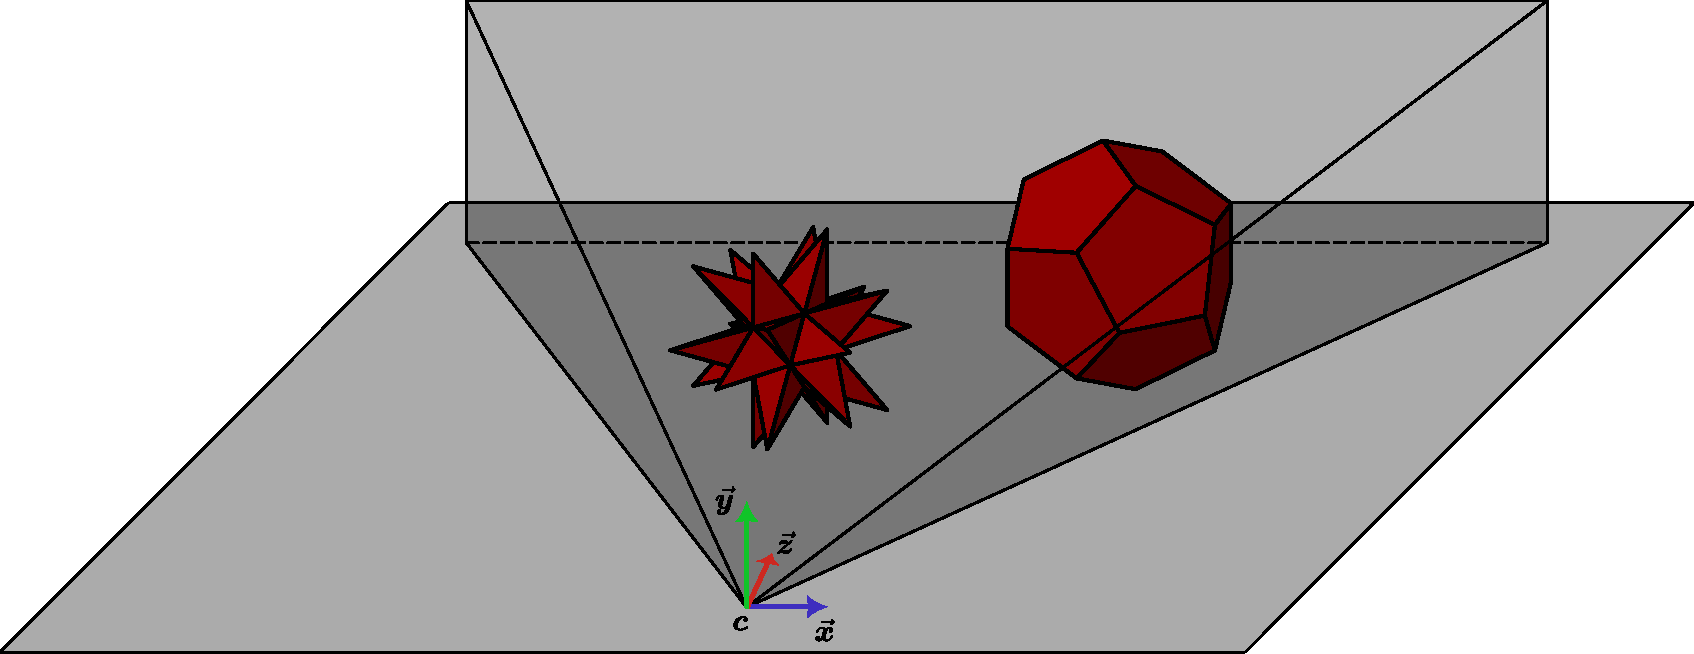
\includegraphics[width=0.95\textwidth]{imagenes/view_matrix_vectors_diagram.pdf}
    \end{center}
    \caption{Vectores base del espacio de la cámara, $\vec{\bm{x}}$, $\vec{\bm{y}}$, $\vec{\bm{z}}$ y posición $\bm{c}$.}\label{fig:camera_view_matrix_vectors_diagram}
\end{figure}

La matriz de vista se actualiza usando la función \texttt{glm::lookAt} de la
biblioteca GLM:

\begin{lstlisting}[language=C++,caption={Actualización de la matriz de vista en Copper}]
void Camera::update_view_matrix() {
    this->view_matrix = glm::lookAt(
        this->eye,
        this->center,
        this->up
    );
}
\end{lstlisting}

Esta función genera una matriz de 4x4 que realiza una traslación y rotación
para situar el origen de coordenadas en la posición de la cámara y orientar los
ejes de acuerdo a los vectores especificados. Los métodos
\texttt{get\_right()}, \texttt{get\_up()} y \texttt{get\_forward()} permiten
obtener los vectores base del espacio de la cámara directamente desde la matriz
de vista transpuesta.

\subsection{Control de la cámara y actualización de la vista}

La clase \texttt{CameraController} gestiona la interacción del usuario para
modificar la vista de la cámara mediante el ratón y el scroll, permitiendo
rotar, trasladar y acercar/alejar la cámara respecto al centro de la escena. El
controlador calcula la nueva orientación usando cuaterniones y actualiza la
matriz de vista de la cámara en función de los movimientos del usuario.

\begin{lstlisting}[language=C++,caption={Actualización de la vista desde CameraController}]
void CameraController::update_view_matrix() {
    auto matrix = glm::transpose(
        mat4_cast(this->total_rotation)
    );

    auto right = glm::vec3(matrix[0]);
    auto up = glm::vec3(matrix[1]);
    auto view_dir = glm::vec3(matrix[2]);

    auto camera_center = this->center;
    auto translation = glm::vec3(
        glm::dot(right, camera_center),
        glm::dot(up, camera_center),
        glm::dot(view_dir, camera_center));

    matrix[0][3] = translation.x;
    matrix[1][3] = translation.y;
    matrix[2][3] = translation.z - this->radius;

    this->camera->set_view_matrix(glm::transpose(matrix));
}
\end{lstlisting}

\subsection{Paso de la matriz de cámara al shader: Uniforms}

Para que el shader pueda utilizar la información de la cámara, la matriz de
vista se pasa como parte de la estructura \texttt{Uniforms}. En Copper, antes
de cada renderizado, la matriz de vista se actualiza y se copia a los datos de
\texttt{uniformsData}, que luego se transfieren a la GPU:

\begin{lstlisting}[language=C++,caption={Actualización del uniform con la matriz de vista}]
uniformsData.mvp_matrix = this->camera->get_view_matrix();
device.GetQueue().WriteBuffer(uniformsBuffer, 0, &uniformsData, sizeof(Uniforms));
\end{lstlisting}

En el shader (WGSL), se accede a esta matriz a través del binding de
\texttt{Uniforms}:

\begin{lstlisting}[language=C++,caption={Uso de la matriz de cámara en el shader}]
struct Uniforms {
    mvp_matrix: mat4x4<f32>,
    //...
};
@group(0) @binding(0) var<uniform> uniforms: Uniforms;

@fragment
fn fragmentMain(in: VertexOutput) -> @location(0) vec4<f32> {
    let cam = transpose(uniforms.mvp_matrix);
    let right = cam[0].xyz;
    let up = cam[1].xyz;
    let forward = cam[2].xyz;
    let eye = cam[0].w * right + cam[1].w * up + cam[2].w * forward;
    //...
}
\end{lstlisting}

La operación \texttt{transpose(uniforms.mvp\_matrix)} permite extraer los
vectores principales de la cámara desde la matriz de vista, siguiendo la
convención de OpenGL y GLM. \break

\subsubsection{Motivos para utilizar una matriz $4\times4$ en la cámara de Copper}

Aunque el cálculo de los rayos de visión en Copper se realiza utilizando
únicamente los vectores principales de la cámara (derecha, arriba y adelante),
es decir, operando esencialmente en tres dimensiones, la matriz de cámara
(\texttt{view\_matrix}) se mantiene en formato $4\times4$ durante todo el
pipeline, a pesar de poder simplificarse a una matriz $3\times4$. Esta decisión se ha tomado por razones de compatibilidad,
flexibilidad y coherencia con las convenciones de las principales APIs y
bibliotecas gráficas.

La matriz de proyección tradicional en gráficos 3D requiere el uso de coordenadas homogéneas ($x, y, z, w$) y
matrices $4\times4$ para poder representar la perspectiva correctamente\cite{Ahn2008}. Sin
embargo, en Copper, no se aplica una matriz de proyección, si no que el cálculo de la perspectiva se
realiza directamente en el shader, utilizando únicamente los vectores de la
cámara y los parámetros de \texttt{aspect\_ratio} y \texttt{FOV}.

En resumen, \textbf{Copper calcula la perspectiva y el ray tracing únicamente
    en tres dimensiones, pero mantiene la matriz de cámara en formato $4\times4$
    por compatibilidad, facilidad de desarrollo y flexibilidad futura}. Este diseño
permite adaptar el sistema a cambios sin necesidad de reescribir partes
significativas del código y sigue las convenciones del desarrollo gráfico
moderno.
